\section{Linux Power Governors}\label{sec:linux-powergov}

\if 0
\begin{figure}[h]
  \begin{center}
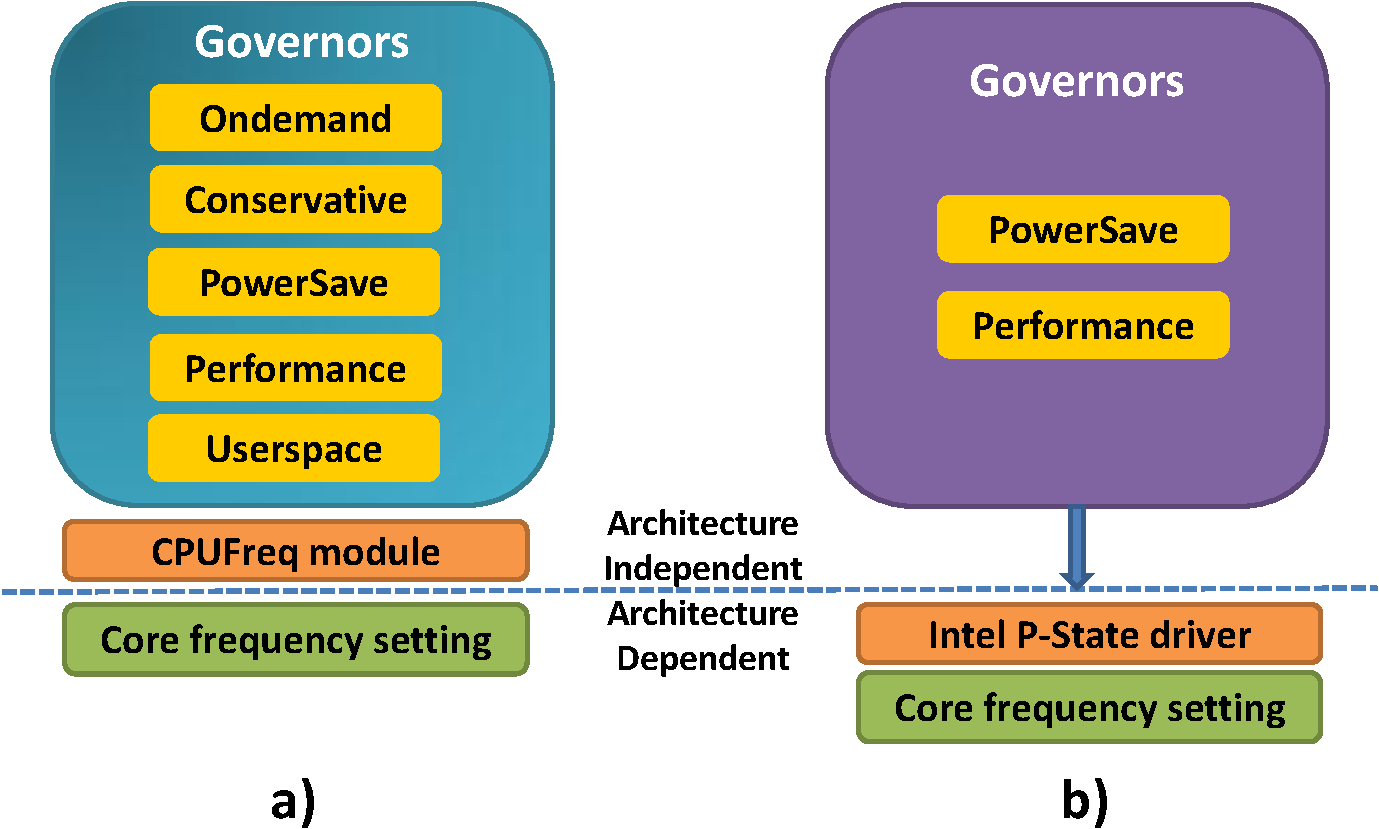
\includegraphics[width=\linewidth]{figs/gov-crop.pdf}
  \end{center}
  \vspace{-0.1in}
  \caption{Freq reduced by 30\%}
	\label{fig:gov}
\end{figure}
\fi

On today's Linux systems, depending on hardware availability and the version of the Linux kernel used in a distribution, power management 
is either handled by the ACPI governors or Intel's P-state drivers. The ACPI governors are platform independent solutions that base their decisions 
on system load and ACPI events and request CPU frequencies. On the other hand, Intel's P-state drivers were introduced in Linux 3.9 and support processors from Sandybridge onwards. 
The P-state drivers are more aware of the hardware capabilities of Intel's processors and request Performance states (P-states) rather than fixed frequencies.

\paragraph{ACPI governors}
These governors attempt to scale the CPU frequency in order to save power. CPU frequencies can be scaled automatically 
depending on the system load, in response to ACPI events, or manually by user space programs. The infrastructure available in Linux kernel to perform 
frequency scaling is called \emph{cpupower}.  

There are a number of ACPI governors available in Linux but the ondemand governor is the most widely used.
This governor sets the CPU frequency depending on the system load.  
In general, this governor tries to run the CPU load at high frequency. If the CPU load placed by the user abates, the Ondemand governor will slowly 
step back down through the kernel's frequency steppings until it settles at the lowest possible frequency, or the user executes another task to demand a ramp.
Ondemand scales its frequency in a work queue context. In other words, once the task that triggered the frequency ramp is finished, 
ondemand will attempt to move the frequency back to minimum. If the user executes another task that triggers ondemand's ramp, the frequency will bounce from minimum to maximum.

\paragraph{P-state drivers}
Intel's P-state drivers work on the race-to-idle concept. Since most modern CPUs consume very little power when idle, these drivers attempt to execute workloads as quickly 
as possible and return the CPU to an idle state. Race-to-idle policies benefit from the power savings of having the CPU in an idle state for most of the time. Apart from 
exploiting the idle CPU power savings, the P-state drivers are also aware of the available Performance states (or P-states), which represent a voltage-frequency operating point for the CPU. 
Currently, two P-state driver algorithms are selectable by the user: powersave and performance. As their names imply, the powersave driver emphasizes power savings at the cost of 
performance while the Performance driver works in a manner that is similar to the ACPI Ondemand governor.
 
\begin{comment}
\subsection{Performance}
This governor sets the CPU statically to a maximum frequency. This governor comes in handy in today’s phones, which implement a faster race to idle. Race-to-idle is the process by which a phone completes a given task, such as syncing email, and returns the CPU to the extremely efficient low-power state. This governor however, relies on a kernel that properly implements low power CPU C states.

\subsection{Powersave}
This governor is the opposite of Performance governor and sets the CPU statically to the lowest frequency set by the user.

\subsection{Userspace}
This governor allows the user or any user space program running with UID “root” to set the CPU to a specific frequency. This governor is more common amongst server and desktop PCs and is seldom used in mobile devices.

\subsection{On Demand}
This governor sets the CPU frequency depending on the current usage. To do this the CPU must have the capability to switch between frequencies very quickly. In general, this governor tries to run the CPU load at high frequency. If the CPU load placed by the user abates, the Ondemand governor will slowly step back down through the kernel's frequency steppings until it settles at the lowest possible frequency, or the user executes another task to demand a ramp.
Ondemand scales its frequency in a work queue context. In other words, once the task that triggered the frequency ramp is finished, ondemand will attempt to move the frequency back to minimum. If the user executes another task that triggers ondemand's ramp, the frequency will bounce from minimum to maximum.
This governor provides tunable parameters like sampling rate, the rate at which governor takes a look at CPU usage and makes a decision about frequency and sampling down factor, the rate at which the governor makes a decision on when to decrease the frequency while running at top speed

\subsection{Conservative}
This governor much like the ondemand governor, sets the CPU depending on the current usage.  It differs in behavior in that it gracefully increases and decreases the CPU speed rather than jumping to maximum speed the moment there is any load on the CPU. This behavior is more suitable in a battery powered environment.
This governor provides tunable parameters like frequency steps, which describes what percentage steps the CPU freq should be increased and decreased smoothly by.

\subsection{Min- Max}
This governor as the name suggests only makes use of minimum and maximum frequencies depending upon the CPU load and does not use any intermediate frequencies.

\subsection{Interactive}
Much like the ondemand governor, the Interactive governor dynamically scales CPU frequency in response to the workload placed on the CPU by the user. However, this governor is significantly more responsive than ondemand, because it's faster at scaling to maximum frequency.
Unlike Ondemand governor, which scales clock speed in the context of a work queue, Interactive governor scales the clock speed over the course of a timer set arbitrarily by the kernel. In other words, if an application demands a ramp to maximum frequency by placing 100\% load on the CPU, an user can execute another task before the governor starts reducing CPU frequency. The timer also renders this governor better suitable to utilize intermediate frequencies.
\end{comment}
